\section{Programs Structure}\label{S_Program}
The files, the directory must contain, are listed in chapter~\ref{SS_1stSteps}. The python code is written in the files  \emph{CPD\_Compos\_and\_Energy.py}, \emph{CPD\_Fit\_lin\_regr.py}, \emph{CPD\_Fit\_one\_run.py} and \emph{Pyrolysis.py}. The last enumerated file controls the whole process. It accesses to the other three files, which contain the corresponding classes with their methods.\\
The figure~\ref{F_Structure} gives a overview of the program structure.\\

proximate analysis~(PA), the ultimate analysis~(UA), both in percent, and the higher heating value~(HHV)

\begin{figure}
\centering%\capstart
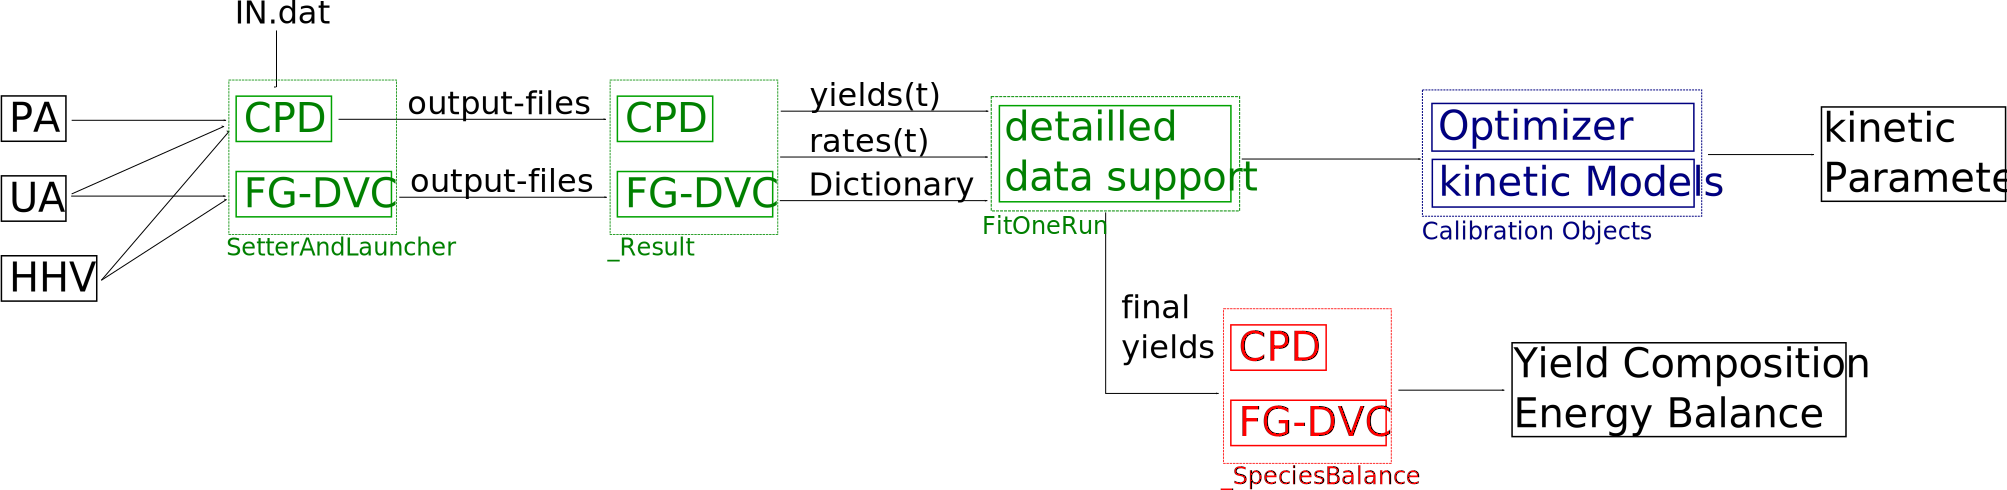
\includegraphics[height=6cm,angle=90]{Figures/Programstructure}
\caption{Overview of the program}
\label{F_Structure}
\end{figure}

\_Result class supports other classes with whole yields and rates Arrays and dictionaries\\
-Dict makes Porgram better to read ('Temp' instead of colnr) and more robust against changes (if another colnr all cols in program had to be changed)\\
-Dict needs only be changed in \_Result\\
-other classes independent from CPD/FG-DVC\\